\documentclass[10pt,a4paper]{article}
\usepackage[left=2cm,right=2cm,top=2cm,bottom=2cm]{geometry}
\usepackage[dvipsnames]{xcolor}
\usepackage[fleqn]{mathtools}
\usepackage{booktabs}
\usepackage{amsmath}
\usepackage{latexsym}
\usepackage{graphicx}
\usepackage{nccmath}
\usepackage{multicol}
\usepackage{listings}
\usepackage{tasks}
\usepackage{color}
\usepackage{float}
\usepackage{lipsum}

\definecolor{colorIPN}{rgb}{0.5, 0.0,0.13}
\definecolor{colorESCOM}{rgb}{0.0, 0.5,1.0}
\graphicspath{ {imagenes/} }

\begin{document}
%#########################################################
\begin{titlepage}
	\centering
	{ \huge \bfseries \color{colorIPN}{Instituto Politécnico Nacional} \par}
	{ \Large \bfseries  \color{colorESCOM}{Escuela Superior de Cómputo} \par }
	\vspace{1cm}
	{\huge\Large \color{colorIPN}{Web App Development}.\par}
	\vspace{1.5cm}
	{\huge\Large  \color{colorESCOM}{Ejercicio 4: Configuración de un DBCP para Acceso a BD PostgreSQL.}\par}
		\vspace{2cm}
	{\Large\itshape \color{colorIPN}{Profesor: M. en C. José Asunción Enríquez Zárate }\par} \hfill \break
	\vspace{2cm}
	{\Large\itshape \color{colorIPN}{Alumno: Chavarría Vázquez Luis Enrique}\par} \hfill \break
	{\Large\itshape \color{colorIPN}{luisechvz@gmail.com}\par} \hfill \break
	{\Large\itshape \color{colorIPN}{3CM4} \par}
	\vfill
	{\large \color{colorIPN}{\today}\par} 
	\vfill
\end{titlepage}

\renewcommand\lstlistingname{Quelltext} 


\lstset{ 
	language=Java,
	basicstyle=\small\sffamily,
	numbers=left,
	numberstyle=\tiny,
	frame=tb,
	tabsize=4,
	columns=fixed,
	showstringspaces=false,
	showtabs=false,
	keepspaces,
	commentstyle=\color{Violet},
	keywordstyle=\color{colorIPN} \bfseries,
	stringstyle=\color{colorESCOM}
}

\settasks{
	counter-format=(tsk[r]),
	label-width=4ex
}
\tableofcontents 
\pagebreak
\listoffigures
\pagenumbering {arabic}

\pagebreak

%################################################
\section{\color{colorIPN}{Introducción}}

Cabe destacar que este ejercicio número iv, se manejará la parte las conexiones abiertas para nuestra base datos de manera que podamos utilizar las a lo largo de múltiples consultas o múltiples actualizaciones, para lo cual implementaremos lo que es conocido en el mercado como pool de conexiones de conecciones, por lo que cuando nosotros utilizamos un programa y nuestro cliente requiere comunicarse con nuestra base datos, demostrable ser una comunicación pero la realidad es que en lo General cuando nosotros utilizamos un cierto protocolo esta conexión pues se utiliza una y otra y otra vez entonces requerimos tener un buen manejo de nuestra conexión a la base datos porque si nosotros podemos reciclar las conexiones de manera efectiva podemos evitar que nuestro sistema se sobrecarga y desde luego ahorrar muchísimo recursos a nivel backend, con el esquema que vamos utilizar podemos generar tareas que tenga múltiples hilos dentro de nuestro programa y poder realizar todo en paralelo de manera mucho más efectiva, el sistema evidentemente se saturar a menos y tenemos un mejor aprovechamiento de todos datos, cuando nosotros mantenemos abierta nuestros conexiones, esto está generando un gasto recursos en el sistema, entonces deberemos usar una manera efectiva de poder administrar todos estos hilos de comunicación con nuestra base datos, cuando estemos utilizando lo evidentemente la conexión se pondrá disposión otro lino que necesite recurso que vamos a poder brindar, por lo cual se asignará un hilo de ejecución; ahora considerando la parte las políticas de grupo ambiental conexiones, todas debemos establecer las conexiones de manera que si en caso de que esto nos ha posible, dejemos atrás el hilo que espera la liberación de alguna conexión para poder mantener todo de manera mucho más eficiente, de modo inverso lo que va a pasar cuando no tenemos múltiples elecciones utilizándose entonces algunas de ellas podrán estar cerradas de manera que podemos optimizar al máximo todo lo que ya hemos mencionado anteriormente y evitar una sobresaturación de nuestros conexiones dentro del sistema, lo cual al final del día se resume en no solamente una mejor optimización sino una mayor seguridad de que el servicio funcionará en todo momento sin absolutamente ningún problema dificultad.



\pagebreak

%################################################
\section{\color{colorIPN}{Conceptos (generalidades)}}


\subsection{JSP.}
Directiva JSP para ajustar toda la página JSP relacionados atributos, tales como la página de codificación y lenguajes de script. Las instrucciones pueden tener una serie de propiedades, que en forma de pares de clave y valor, separados por comas.

\subsection{Aplicación web.}
En la Ingeniería de software se denomina aplicación web a aquellas aplicaciones que los usuarios pueden utilizar accediendo a un Servidor web a través de Internet o de una intranet mediante un navegador.

\subsection{SERVLETS.}
Un servlet es una clase en el lenguaje de programación Java, utilizada para ampliar las capacidades de un servidor. ... El uso más común de los servlets es generar páginas web de forma dinámica a partir de los parámetros de la petición que envíe el navegador web.

\subsection{JDBC.}
JDBC proporciona Controladores JDBC que convierte la solicitud de la aplicación Java en el lado del cliente al lenguaje que entiende la base de datos. Como JDBC es específico del idioma y la plataforma, la aplicación Java puede usar JDBC a ODBC puente para comunicarse con bases de datos adaptables ODBC.

\subsection{Driver manager.}
La clase DriverManager implementa la capa de gestión de JDBC, y trabaja como intermediaria entre el usuario y los drivers. Guarda la lista de los drivers que están disponibles y establece la conexión entre la base de datos y el driver apropiado.

\subsection{Conectores.}
Es un estándar de acceso a las bases de datos desarrollado por SQL Access Group en 1992. El objetivo de ODBC es hacer posible el acceder a cualquier dato desde cualquier aplicación, sin importar qué sistema de gestión de bases de datos (DBMS) almacene los datos.



\pagebreak

%################################################
\section{\color{colorIPN}{Desarrollo y resultados}}


En el desarrollo este ejercicio iremos describiendo los pasos necesarios para poder configurar todo nuestro recursos y desde luego también tener en línea todos nuestros archivos necesarios para poder hacer la creación y poder permitirnos tener nuestras conexiones todas de manera estable de manera que podamos optimizar todo de manera lo más eficiente posible dentro de nuestra aplicación utilizando los recursos que vemos a continuación.
\vspace{5mm}

Primero que nada debemos crear nuestro proyecto o, para lo cual estaremos trabajando en este caso con la base datos creada en postgresql, con lo cual ya podemos dar rienda suelta a la parte la configuración de nuestro servidor, para ello debemos definir primero directorio de nuestro editor de texto para mi caso yo lo voy a ser directamente en que viene siendo visual studio. Ahora bien, el recurso va ser definido acorde con lo que ya conocíamos va después de toda la parte el etiquetado recursos globales, y también tenemos que hacer la parte los recursos previamente vamos utilizar también para generar un recurso ya sea en nuestro gestor, también dentro del cuerpo del etiqueta tenemos que modificar algunos de los parámetros, pero en sí lo que tenemos indicar es que en la parte las conexiones nosotros vamos utilizar nuestro controlador jdbc/postgres con lo cual polla procedemos directamente a atender la parte el trabajo con nuestra base y también indicar la parte la conexión lleva que vamos utilizar directamente nuestro base datos con postgres, con lo cual polla nada más indicamos la dirección, posteriormente acorde con el orden de la url tenemos que indicar la parte de nuestro puerto y finalmente tenemos que simplemente conectarlo la base datos, pero para esto es importante que indique moda dirección de pues ya simplemente llamamos al proyecto. Con lo cual pues ésta sería la parte definición de los parámetros que debemos utiliza para modificar nuestro servidor, es importante que hagamos un reinicio del sistema, en mi caso yo lo incitó a mi computadora para poder asegurar que los cambios se llevarán a cabo porque ya lab intentado sin reiniciar y puede ser el resultado un poco desastroso ya que no se vieron a dos absolutamente ningún cambio, y ya posteriormente vamos utilizar simplemente nuestro sistema de la manera tradicional en la que estamos acostumbrados.
\vspace{5mm}
\begin{figure}[h]
\centering
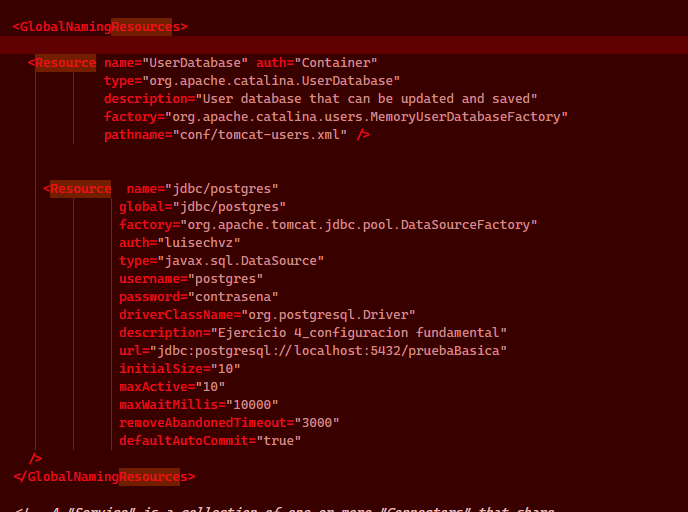
\includegraphics[width=7cm]{1XX}
\caption{Configuración de los recursos para el server.}
\label{fig:re1}
\end{figure}


Ya posteriormente lo único que tenemos que hacer es descargar nuestro jar de postgres para poder poner la nuestro sistema, básicamente lo único que tenemos que hacer es irnos a conectarnos a la parte la carpeta configuraciones y pues básicamente ya una vez que ese modo descarga de nuestro archivo ya nada más vamos a la parte de lib de nuestro server el cual en mi caso yo estoy empleando tomcat en su ultima versión y pues ya simplemente es una cuestión de colocar el archivo que hemos descargado directamente de la página de postgres y colocarlo directamente nuestro sistema para que esto quede concluido de manera satisfactoria cabe destacar que yo lo hice en el sistema operativo windows de la empresa microsoft en su versión número diez con lo cual este proceso probablemente pueda cambiar de un sistema otro, por lo cual yo nos garantizó que esto vaya funcionando los sistemas pero al menos en mi o si funciono.
\begin{figure}[h]
\centering
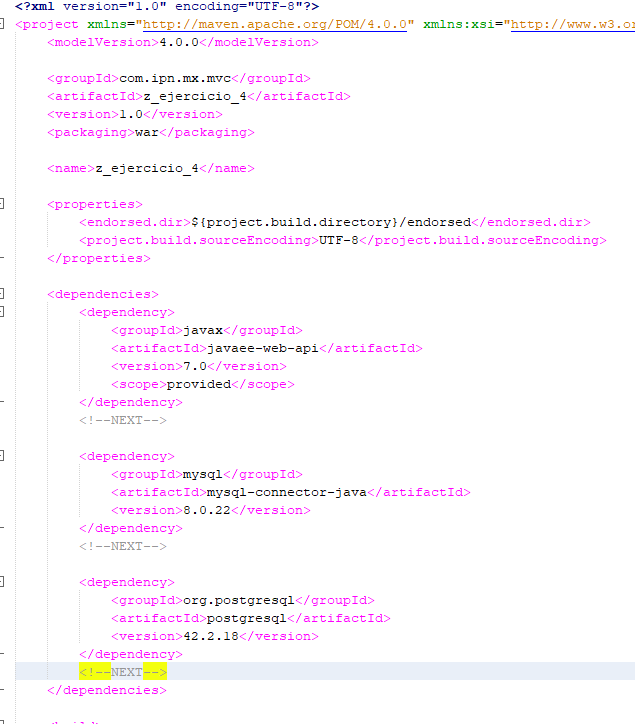
\includegraphics[width=6cm]{2XX}
\caption{Configuración de nuestra dependencias.}
\label{fig:re1}
\end{figure}
\vspace{60mm}

Ahora bien pues ya una vez hecho esto simplemente basta poder empezar a trabajar con la aplicación que ya habíamos creado de manera previa, el cual pues lo vamos a trabajar en el mismo editor de texto que hemos está utilizando durante todo estas prácticas y basta con que simplemente creemos nuestro proyecto como ya lo conocíamos anteriormente pero ahora que vincularlo con un archivo para la parte de postgres y todo manejo de la base datos, ya que bueno en este caso tenemos ubicado todo con respecto un nombre, y tenemos que hace que se despliegue en la pantalla toda la lista los repositorios que tenemos disponibles por el momento por lo cual simplemente basta con acceder a ellos y poder acceder a nuestro código sin ningún problema ahora bien también es necesario que directamente nuestro archivo de configuración en vayamos y agregamos la dependencia de postgres ya que sin esto pues al momento de construir nuestro proyecto con las dependencias sino lo agregamos evidentemente proyecto se va a construir sin ellas, por lo cual es tan simple como simplemente ir y pegar la parte que han establecido para el manejador de archivos maven directamente en la parte la configuración de las des pendencias hipódromo subir nuestro proyecto con postgres sin absolutamente ningún problema.
\begin{figure}[h]
\centering
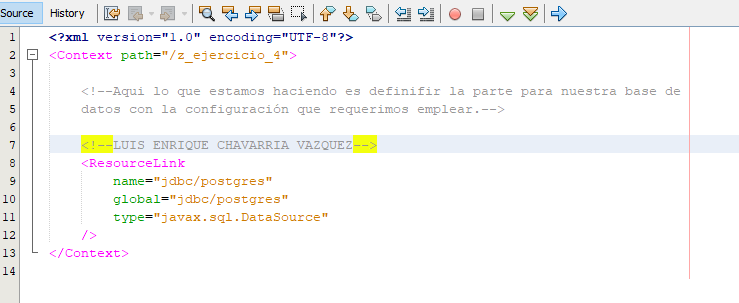
\includegraphics[width=13cm]{3XX}
\caption{Eliminación de los datos.}
\label{fig:re1}
\end{figure}



Ya simplemente falta que nosotros vayamos a configurar nuestra archivo de contexto para qué bueno todas las carpetas queden de manera vinculadas de forma correcta y esto basta de la parte los metadatos o meta-información, con lo cual ya podemos proceder directamente trabajar con nuestros recursos de la fuente y con todo esto o pues simplemente trabajar con la parte de nuestro controlador de la base datos, cabe declara que para esto necesitamos detener una base de datos creada para poder tener lamentación de la forma correcta y adecuada; porque en caso de que en un sistema base datos que nos puede ayudar a gestionar to esta parte pues tendremos algunos problemas a la hora de poder entablar comunicación con ella ya que en existe o al menos de que ya llamo subido una base de datos a la plataforma como puede ser Heroku para poder establecer esta conexión directamente con la base de datos ya creada o algún tipo de server que nos puede ayudar a establecer dicha comunicación y obtener los datos de manera remota, pero en este caso al inicio se tiene que hacer la prueba de manera local para poder garantizar el correcto funcionamiento con el manejador de las bases de datos que hemos definido.
\begin{figure}[h]
\centering
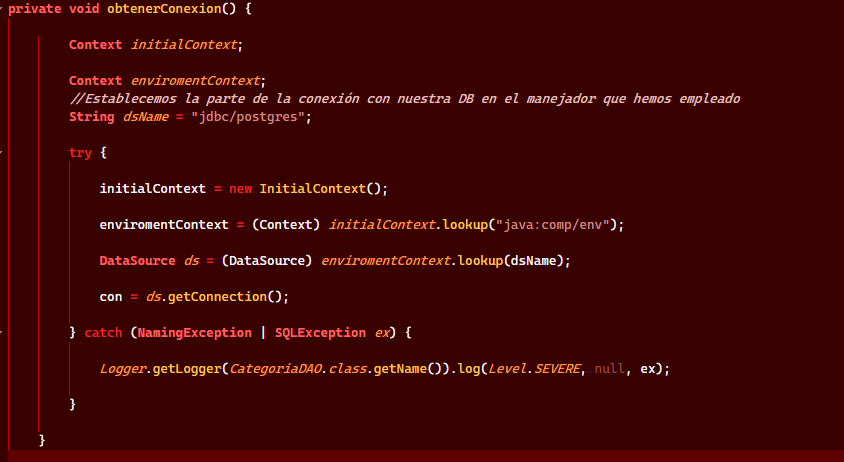
\includegraphics[width=12cm]{4XX}
\caption{Agregación de los usuarios.}
\label{fig:re1}
\end{figure}
\vspace{160mm}



Para la parte de la configuración de la obtención de la conexión, es tan sencillo como simplemente configurarlo en nuestro gestor de los archivos del modelado y ya posteriormente dentro de las categorías modificamos la parte de la conexión que vamos a realizar y pues ya sólo es cuestión de poder modificarlo de acuerdo nuestras necesidades, dependiendo del tipo de manejador de bases de datos que utilizamos evidentemente esto cambiará de tanto en tanto o simplemente tenemos que establecer una configuración distinta dependiendo de los manejadores que vallamos emplear durante todo este proceso como para lo cual yo simplemente quiero decir que bueno en este caso postgres ha demostrado ser un manejador de base de datos bastante eficiente muy bueno que puede competir en efecto, el tipo de manejador de base datos y además nos ofrece muchísimas ventajas a nivel técnico.
\begin{figure}[h]
\centering
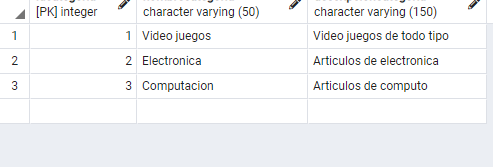
\includegraphics[width=8cm]{5XX}
\caption{Editar usuarios.}
\label{fig:re1}
\end{figure}

Ahora bien ya directamente nosotros podamos hacer una selección de los elementos en nuestra base datos y podemos ver toda la información, para lo cual pues simplemente basta con que nosotros hagamos una selección de las categorías y podamos ver lo en pantalla para que evidentemente toda la información de dichas categorías puede desplegarse sin absolutamente ningún problema.
\vspace{160mm}

\pagebreak



%################################################
\section{\color{colorIPN}{Conclusión}}
\vspace{5mm}
Puedo concluir que a lo largo de este ejercicio he aprendido a realizar de manera eficiente toda la parte la configuración de los recursos que vamos utilizar durante el proceso de reelaboración de nuestras bases de datos, lo cual es bastante bueno porque al final del día trabajar con ese tipo optimización en nos ayudan a poder tener mucha más ventajas al momento desarrollar y desde luego para distintos patrones de desarrollo que nos da la pauta para codificar y tener mejores prácticas de desarrollador con lo que se refiere a nuestras bases de datos, ahora bien se me presentaron varias dificultades durante este proceso de elaboración de el desarrollo de este ejercicio número 4 que hemos arrollado; quiero destacar también otra parte que considero bastante importante y es que usualmente toda mi vida yo vi estado trabajando con otro tipo de manejadores de bases de datos en su mayoría han de tipo uno relacional, también había estado trabajando mucho con firebase y en especial en el lado de la parte de manejo con base de datos relacionales había estado trabajando muchísimo con la parte de mysql, pero ahora me he dado la oportunidad está trabajando con este gestor de base datos que es un poco diferente pero que también ofrece mucha más ventajas y sobre todos mucho más ligero; la verdad es que este tipo experiencia sí ayudan bastante a la experiencia desarrollo y a poder trabajar de manera mucho más oportuna con otro tipo de manejadores que igual y nos podemos encontrar industry que nos puedan una gran ventaja al momento está trabajando en un empresa que evidentemente utilice estos servicios y posteriormente nosotros podamos adaptarlo para poder obtener mejores resultados en nuestro trabajo, nivel profesional o inclusive en algun desarrollo tecnológico que nosotros estamos implementando manera de negocio servicio.


\pagebreak

%################################################

\section{\color{colorIPN}{Referencias Bibliográficas}}
\color{colorESCOM}{
	\begin{thebibliography}{10}
	
				\bibitem[GeeksforGeeks, 2020]{GeeksforGeeks}
		Introduction to servlets
		\newblock {\em shorturl.at/ciIMU}
		\newblock GeeksforGeeks, 2020.

\bibitem[JAVA T POINT, 2020]{JAVA T POINT}
		JAVA T POINT
		\newblock {\em https://www.javatpoint.com/servlet-tutorial}
		\newblock JAVA T POINT, 2020.

\bibitem[vogella, 2020]{vogella}
		Introduction to Java Web development.
		\newblock {\em https://www.vogella.com/tutorials/JavaWebTerminology/article.html}
		\newblock vogella, 2020.


	\end{thebibliography}
}

\pagebreak


\end{document}
